\documentclass[a4paper]{article}
\usepackage[english]{babel}
\usepackage[utf8x]{inputenc}
\usepackage{amsmath}
\usepackage{graphicx}
\usepackage[colorinlistoftodos]{todonotes}
\usepackage{listings}
\usepackage{cite}
\usepackage{glossaries}
\usepackage[
top    = 2.75cm,
bottom = 2.00cm,
left   = 2.50cm,
right  = 2.00cm]{geometry}

\title{Remoting Patterns}

\author{Haidn, Siegel}

\date{\today}

\begin{document}
\maketitle
\newpage

\tableofcontents
\newpage

\section{Aufgabenstellung}
Gruppenarbeit: 2 Mitglieder (Server/Client)\\
\\
Analysieren Sie in einer Gruppe von 2 Leuten die mitgelieferte Implementation der verteilten LeelaApplikation. Identifizieren Sie dabei alle verwendeten Elemente der "Basic Remoting Patterns" und erstellen Sie UML-Klassendiagramme für die Pakete comm, comm.socket, comm.soap, evs2009 und evs2009.mapping.\\
Schließen Sie die unfertigen Tests ab, und dokumentieren Sie etwaige Schwierigkeiten.\\
\\
\textbf{Was ist zu tun?}
\begin{itemize}
	\item UML Klassendiagramm
	\item Erweitern der Testfälle (mind. einen Testfall erweitern)
	\item Kritik und Verbesserungsvorschläge
\end{itemize}
\mbox{} \\
\textbf{Punkte (16):}\\
Identifikation von Basic Remoting Patterns ... 1Pkt\\
Beschreibung der Applikation ... 4Pkt\\
UML-Diagramme ... 3Pkt\\
Schreiben von einem neuen Testfall ... 2Pkt\\
konstruktive Verbesserungsvorschläge / Kritikpunkte ... 6Pkt\\
\\
\textbf{Main-Method-Classes}\\
\begin{center}
	\begin{tabular}{ | r | r |}
		\hline
		SOAPPluginServer & src/main/java/comm/soap/SOAPPluginServer.java \\
		\hline
		Application & src/main/java/evs2009/Application.java \\
		\hline
	\end{tabular}
\end{center}

\newpage
\section{Einleitung}
\subsection{Allgemein}
Design Patterns haben in den letzten Jahren eine bedeutende Rolle in der objektorientierten\\
Softwareentwicklung bekommen.\\
Ein Pattern ist mit einer Drei-Punkte-Regel zu vergleichen und setzt sich aus den folgenden Komponenten zusammen:
\begin{itemize}
	\item Kontext
	\item Problem
	\item Lösung
\end{itemize}
Ziel und Nutzen eines Patterns soll es sein Software zu entwickeln, der es möglich ist sich soweit selbst zu konfigurieren,
dass interne Prozesse auf ein sich änderndes Umfeld angepasst und optimiert werden können.\\
\subsection{Verteilte Systeme}
Im gebiet der verteilten Systeme kommen allerdings ein paar weiterte Herausforderungen auf uns zu.\\
Folgenden Herausforderungen schenken wir hierbei unser Augenmerk:
\begin{itemize}
	\item Network Latency
	\item Predictability
	\item Concurrency
	\item Scalability
	\item Partial Failure
\end{itemize}
\begin{center}
	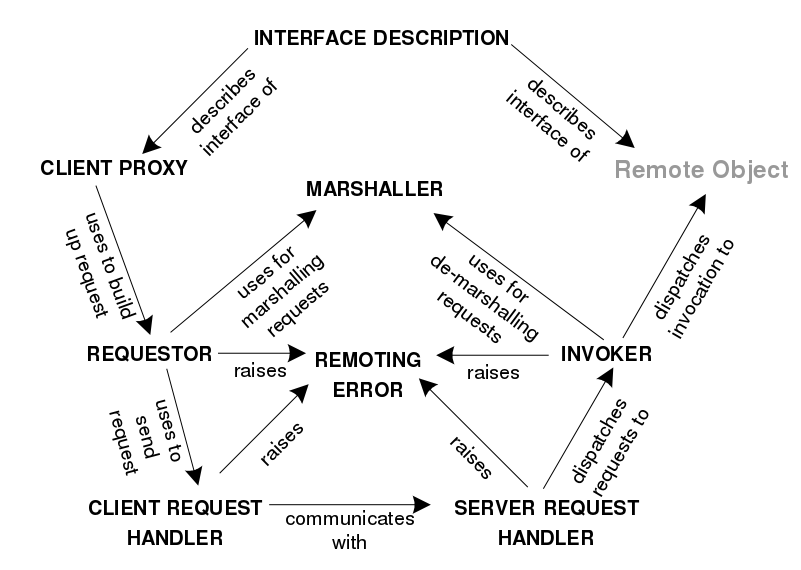
\includegraphics[scale=0.4]{img/remoting_patterns.png}
\end{center}
Die dick gedruckten Knotenpunkte in der obigen Grafik, beschreiben bereits unsere Remoting Patterns.\\
Im Zuge dieser Übung haben wir uns mit dem LeelaApplikation-Framework auseinandergesetzt und den Code auf Basic Remoting Patterns untersucht.\\
Eine detailierte Übersicht folgt im nächsten Punkt.
\cite{RP-WU-Wien}

\newpage
\section{Beschreibung der Applikation}
Die Hauptklasse des Programmes stellt \textbf{Application.java} dar, in der über den PeerReader alle Peer-ID's und die dazugehörigen Adressen eingelesen werden.\\
Für den lokalen Test der Applikation wurden diese Adressen auf "localhost" gesetzt.\\
\\


\section{UML}
Eine Bessere Qualitaet der Diagramme finden sich in der Abgabe. \\ Sie wurden folgendermassen mittels Astah generiert: \\ \\
\begin{itemize}
\item New Project 
\item 
\item
\end{itemize}
	\subsection{comm}
	\begin{figure}[here!]
	\centering
	\includegraphics[width=0.8\textwidth]{comm.png}
	\caption{UML of the comm package}
	\end{figure}
	\subsection{comm.socket}
	\begin{figure}[here!]
	\centering
	\includegraphics[width=0.8\textwidth]{client.png}
	\caption{UML of the soap package}
	\end{figure}
	\subsection{comm.soap}
	\begin{figure}[here!]
	\centering
	\includegraphics[width=0.8\textwidth]{socket.png}
	\caption{UML of the socket package}
	\end{figure}
	\subsection{evs2009}
	\begin{figure}[here!]
	\centering
	\includegraphics[width=0.8\textwidth]{socket.png}
	\caption{UML of the evs2009 package}
	\end{figure}
	\subsection{evs2009.mapping}
	\begin{figure}[here!]
	\centering
	\includegraphics[width=0.8\textwidth]{socket.png}
	\caption{UML of the soap package}
	\end{figure}
\section{Testfälle}
\section{Kritik und verbesserungsvorschläge}
	\begin{itemize}
		\item Der erste Kritikpunk ist die nicht vorhandene Dokumentation des Programmes.\\
		Zumindest ein kleines Kommentar zur Beschreibung der Klasse wäre eine große Hilfe gewesen, sich schneller im Code zurecht zu finden.
		
	\end{itemize}

\newpage
\bibliography{sources}{}
\bibliographystyle{alpha}
		
\end{document}
